%! TEX root = main.tex

Before we use the cases in the first group for further benchmarking, we examine some results in this section.
We present the training histories and visualizations for the cases with the best, median, and worst $L_{2,sp-t}$ of $u$ velocity.
These cases correspond to $(N_l, N_n, N_{bs}) = (3, 256, 4096)$, $(2, 32, 65536)$, and $(1, 32, 16384)$, respectively.
And their $L_{2,sp-t}$ are $8.3e-3$, $1.4e-1$, and $3.1e-1$.
In the following discussion, we will use the format of $(N_l, N_n, N_{bs})$ to refer to the specific case we are discussing.

\begin{figure}[hbt!]
\centering%
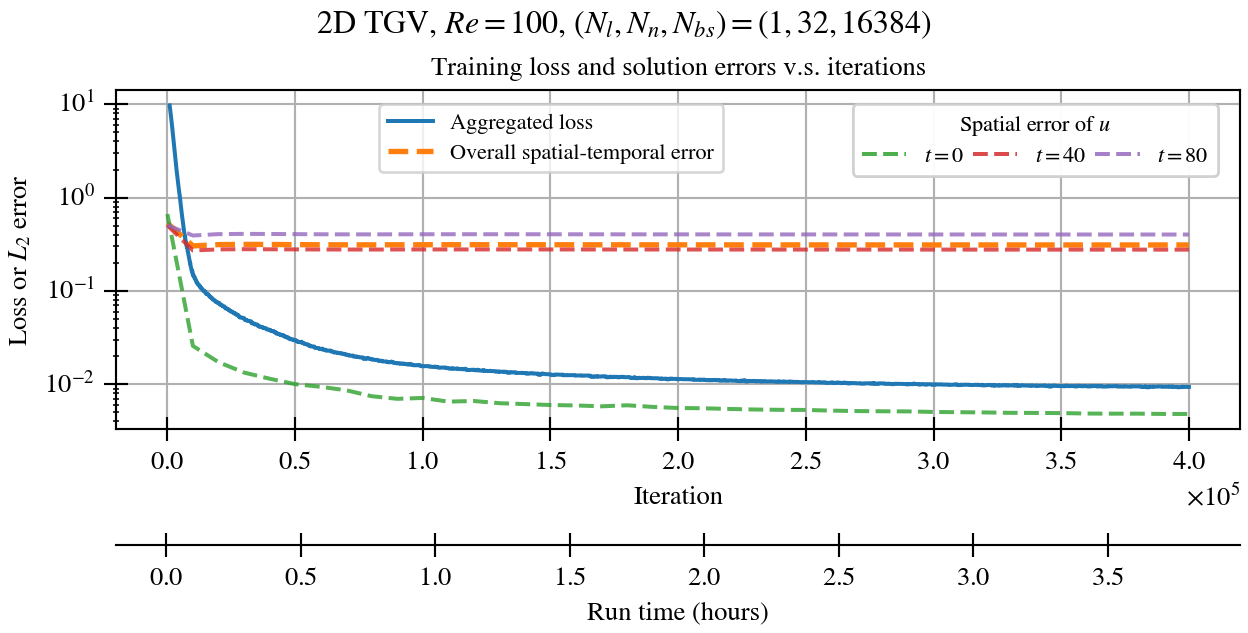
\includegraphics[width=0.9\linewidth]{tgv-2d-re100/training-hist/nl1-nn32-npts16384}%
\caption[%
    Aggregated loss and $L_2$ errors of $u$ v.s. iterations ($(N_l, N_n, N_{bs})=(1, 32, 16384)$)%
]{%
    Aggregated loss and $L_2$ errors of $u$ v.s. iterations ($(N_l, N_n, N_{bs})$ $=$ $(1, 32, 16384)$)%
}\label{fig:nl1-nn32-npts16384-loss-err-hist}%
\end{figure}

\begin{figure}[hbt!]
\centering%
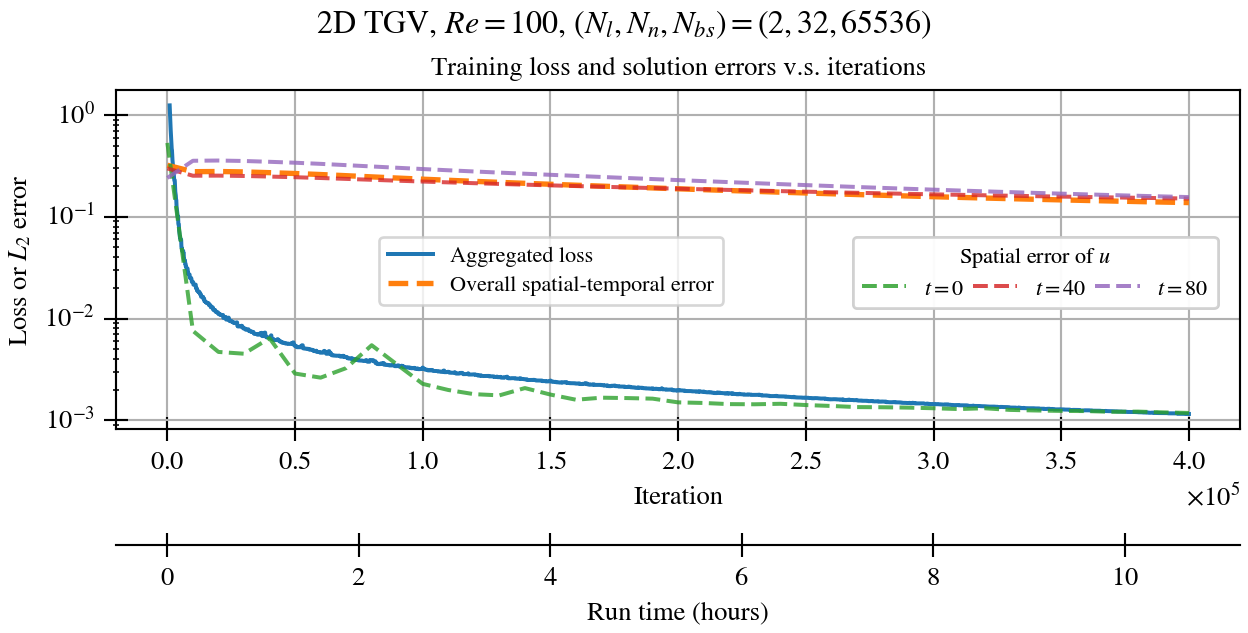
\includegraphics[width=0.9\linewidth]{tgv-2d-re100/training-hist/nl2-nn32-npts65536}%
\caption[%
    Aggregated loss and $L_2$ errors of $u$ v.s. iterations ($(N_l, N_n, N_{bs})=(2, 32, 65536)$)%
]{%
    Aggregated loss and $L_2$ errors of $u$ v.s. iterations ($(N_l, N_n, N_{bs})$ $=$ $(2, 32, 65536)$)%
}\label{fig:nl2-nn32-npts65536-loss-err-hist}%
\end{figure}

\begin{figure}[hbt!]
\centering%
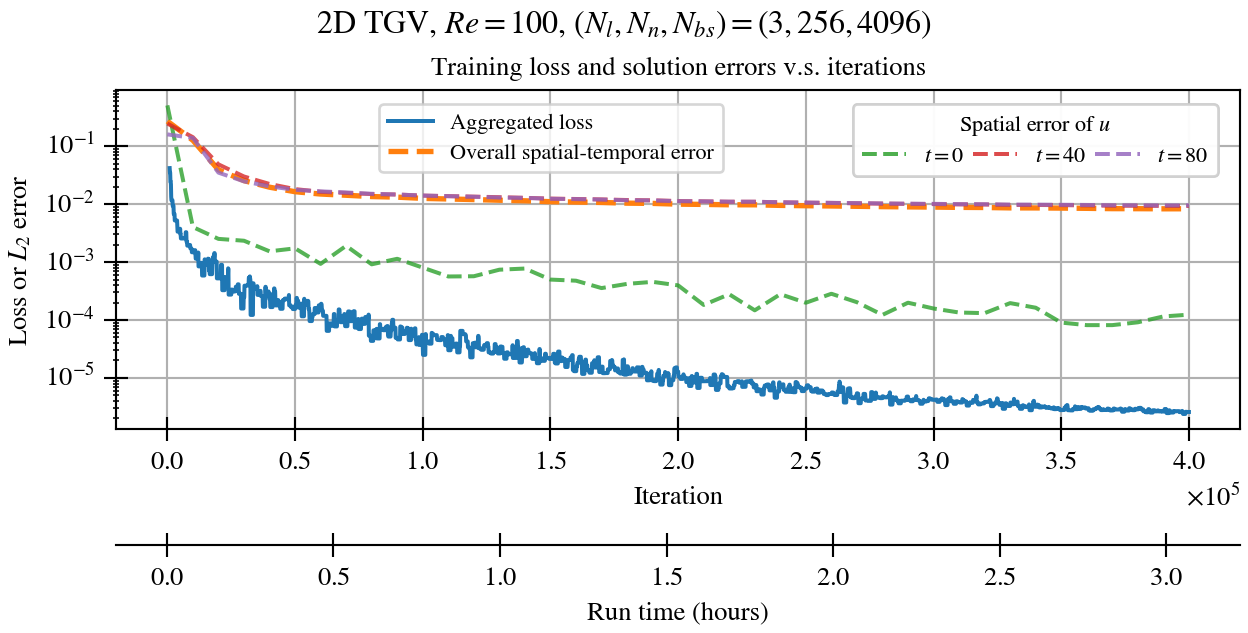
\includegraphics[width=0.9\linewidth]{tgv-2d-re100/training-hist/nl3-nn256-npts4096}%
\caption[%
    Aggregated loss and $L_2$ errors of $u$ v.s. iterations ($(N_l, N_n, N_{bs})=(3, 256, 4096)$)%
]{%
    Aggregated loss and $L_2$ errors of $u$ v.s. iterations ($(N_l, N_n, N_{bs})$ $=$ $(3, 256, 4096)$)%
}\label{fig:nl3-nn256-npts4096-loss-err-hist}%
\end{figure}

Figures \ref{fig:nl1-nn32-npts16384-loss-err-hist}, \ref{fig:nl2-nn32-npts65536-loss-err-hist}, and \ref{fig:nl3-nn256-npts4096-loss-err-hist} show how the aggregated loss $L_{2,sp-t}$, $L_2@t=0$, $L_2@t=40$, and $L_2@t=80$ for $u$ velocity progressed with training iterations.
A second $x$ axis at the bottom of these figures shows the corresponding run time (in hours).

Only the aggregated loss of $(1, 32, 16384)$ obviously converged, and the other two still show some potential to reach a smaller loss.
However, if we examine the history of $L_{2,sp-t}$, $L_2@t=40$, and $L_2@t=80$, the trends of these errors do not show much potential for improvement.
Especially from the case of $(3, 256, 4096)$, we see that the errors of $u$ does not change significantly after 200,000 iterations.
More training iterations only improve the error at $t=0$.
Note that the solution at $t=0$ is determined by the IC losses only, meaning the correct solution at $t=0$ is given to PINNs.
The solutions of $t=40$ and $t=80$ are mainly affected by PDE losses, and the PINNs do not have correct solutions.
The results shown in these figures mean that PINNs in this benchmark are only able to learn well from where we already provide explicit and correct answers.
PINNs do not perform well on solving the actual PDEs, where the solutions are unknown to them.
And learning well on IC does not help in solving the PDEs.

\begin{figure}[hbt!]
    \centering%
    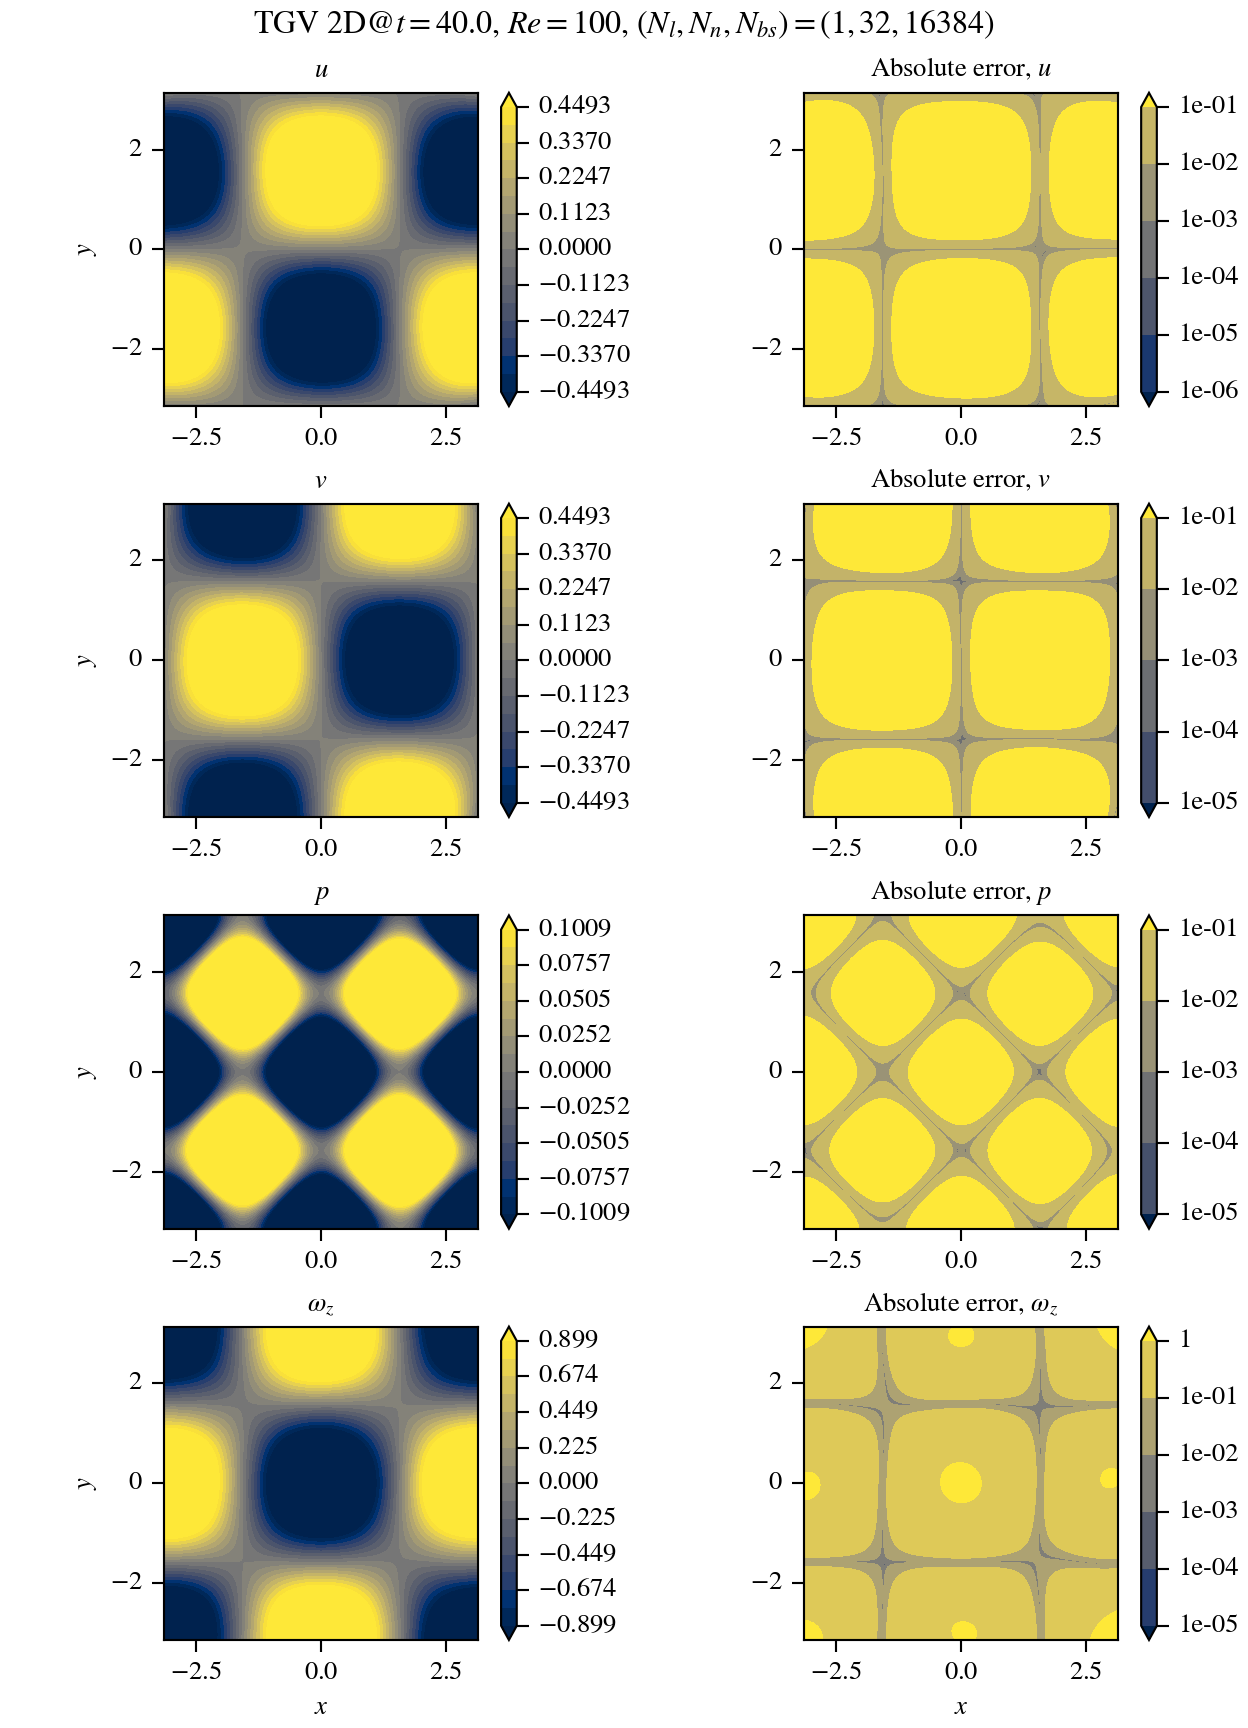
\includegraphics[width=0.9\linewidth]{tgv-2d-re100/contours/nl1-nn32-npts16384-t40.0.png}
    \caption[%
        Predictions and error contours at $t=40$ for $(N_l, N_n, N_{bs})=(1, 32, 16384)$%
    ]{%
        Predictions and error contours at $t=40$ ($(N_l, N_n, N_{bs})$ $=$ $(1, 32, 16384)$)%
    }
    \label{fig:nl1-nn32-npts16384-t40-contours}
\end{figure}

\begin{figure}[hbt!]
    \centering%
    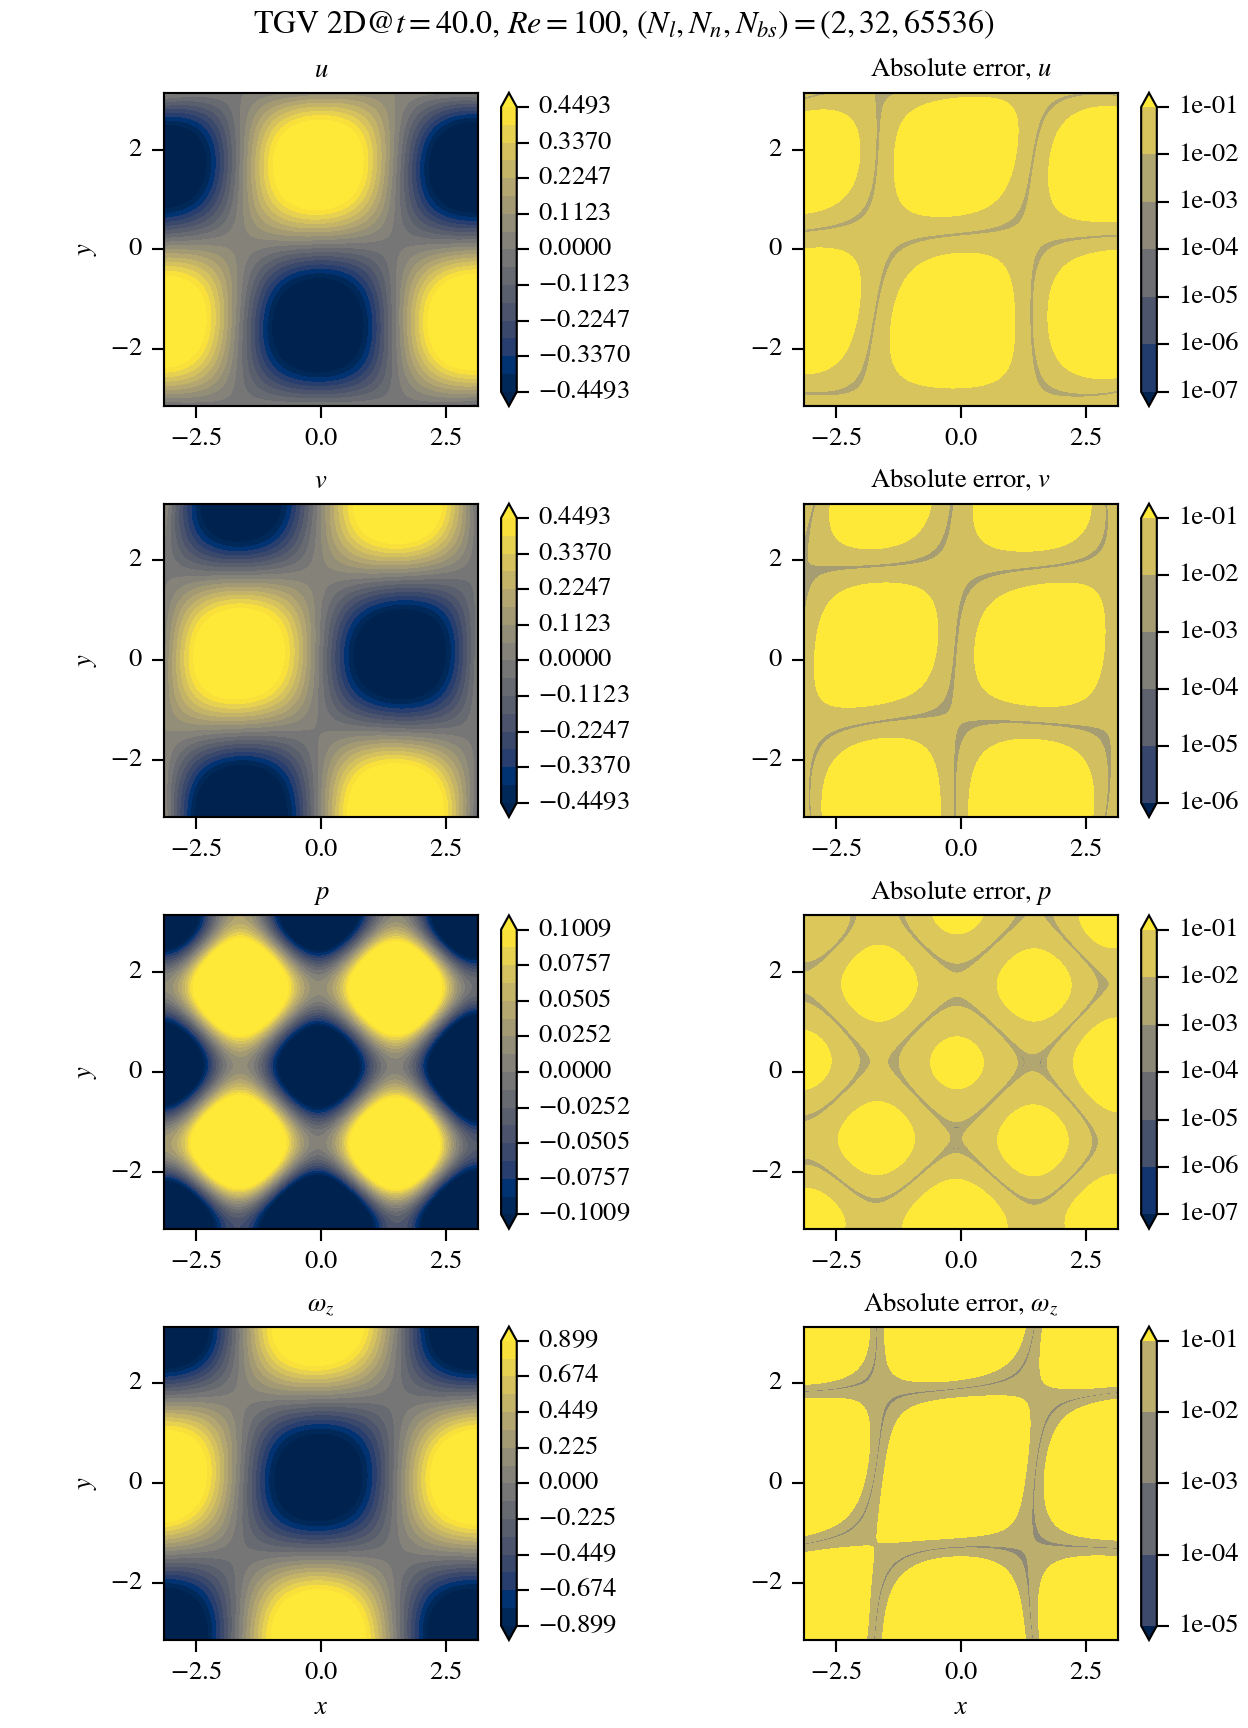
\includegraphics[width=0.9\linewidth]{tgv-2d-re100/contours/nl2-nn32-npts65536-t40.0}
    \caption[%
        Predictions and error contours at $t=40$ for $(N_l, N_n, N_{bs})=(2, 32, 65536)$%
    ]{%
        Predictions and error contours at $t=40$ ($(N_l, N_n, N_{bs})$ $=$ $(2, 32, 65536)$)%
    }
    \label{fig:nl2-nn32-npts65536-t40-contours}
\end{figure}

\begin{figure}[hbt!]
    \centering%
    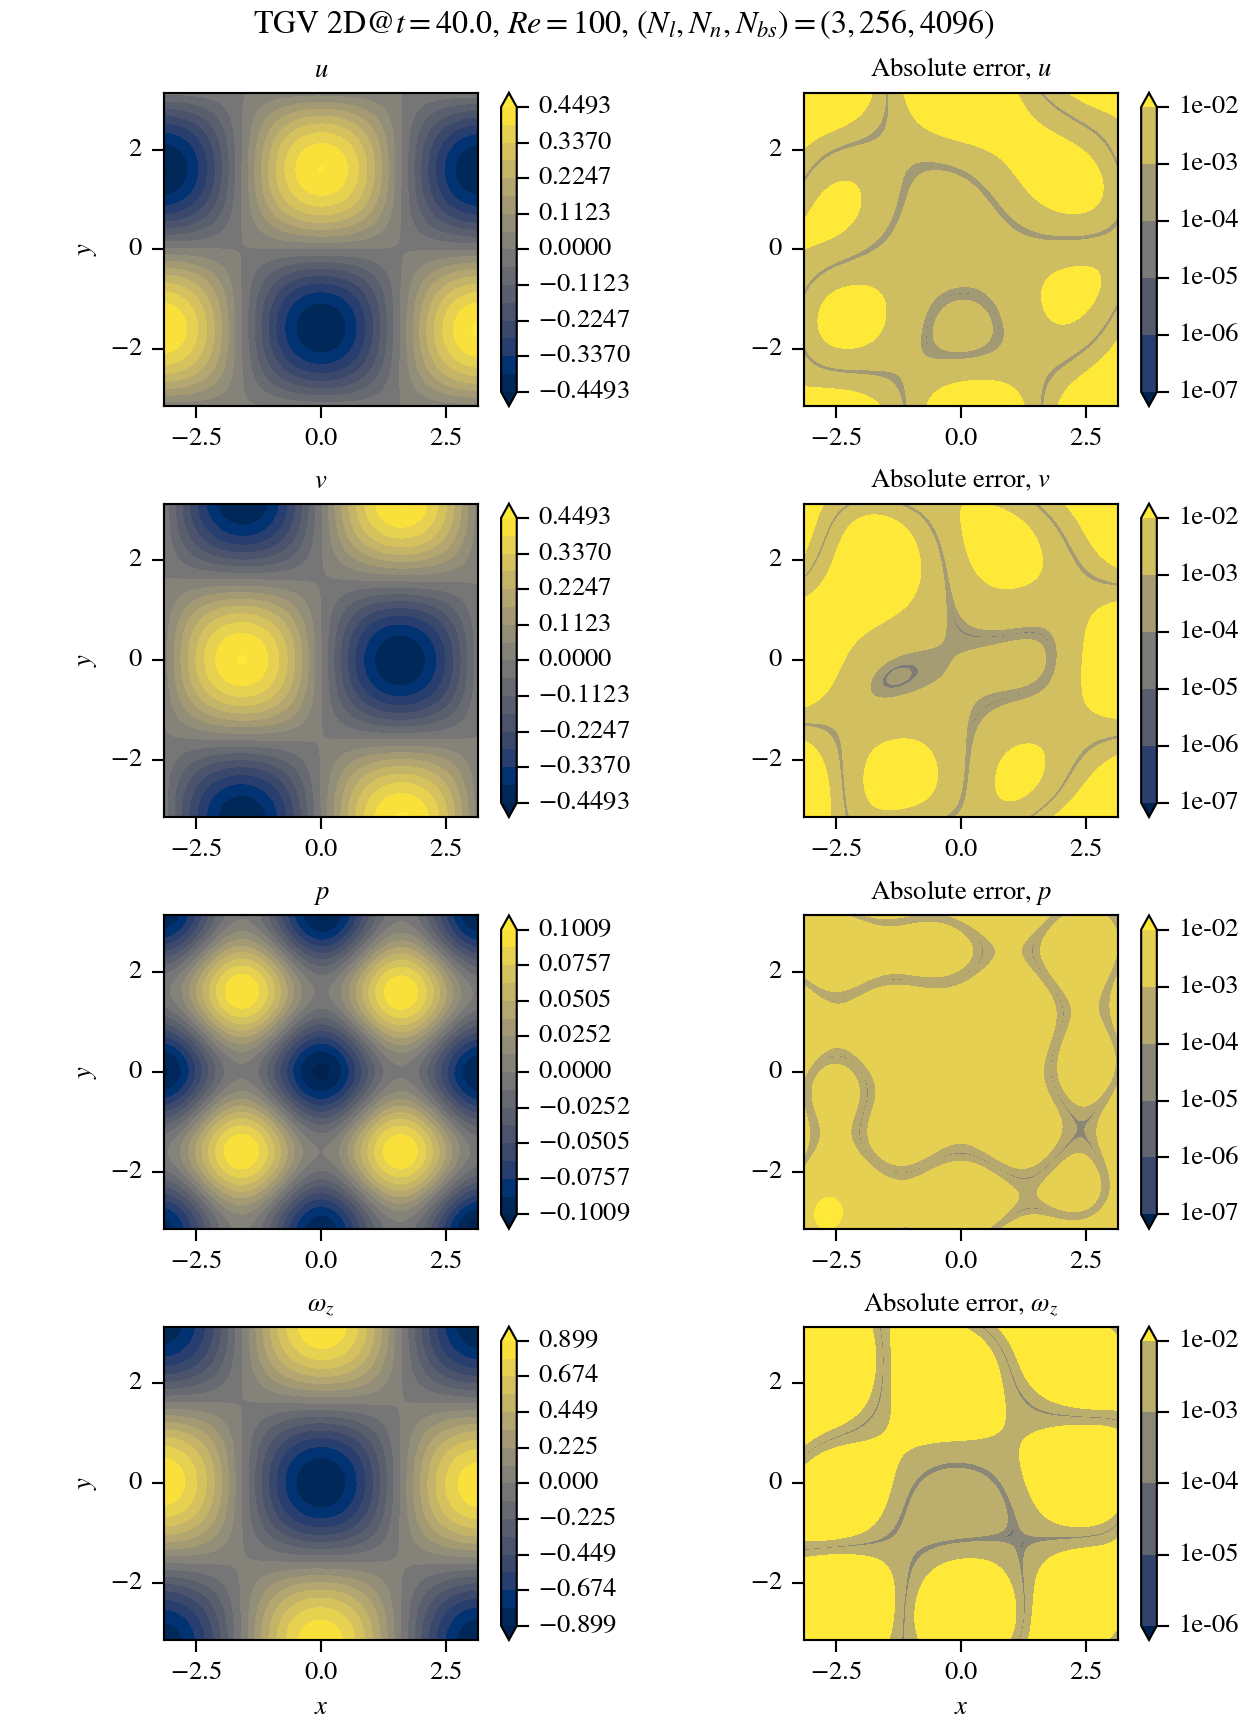
\includegraphics[width=0.9\linewidth]{tgv-2d-re100/contours/nl3-nn256-npts4096-t40.0.png}
    \caption[%
        Predictions and error contours at $t=40$ for $(N_l, N_n, N_{bs})=(3, 256, 4096)$%
    ]{%
        Predictions and error contours at $t=40$ ($(N_l, N_n, N_{bs})$ $=$ $(3, 256, 4096)$)%
    }
    \label{fig:nl3-nn256-npts4096-t40-contours}
\end{figure}

If we compare the run times, the case of $(2, 32, 65536)$ took the longest, about 10.5 hours.
The case of $(1, 32, 16384)$ and $(3, 256, 4096)$ took about 3.8 and 3 hours, respectively.
Intuitively speaking, this observation shows that the run times are mainly dominated by the numbers of training points per batch rather than the complexity of a network.

We also compare the final $L_{2,sp-t}$ from the three cases with that in figure \ref{fig:petibm-tgv-spatial-temporal-error}.
While PetIBM was able to achieve an error level of $10^{-3}$ in less than 20 seconds, none of the three PINN cases was able to achieve the same level of error-cost ratio.

Figures \ref{fig:nl1-nn32-npts16384-t40-contours}, \ref{fig:nl2-nn32-npts65536-t40-contours}, and \ref{fig:nl3-nn256-npts4096-t40-contours} show the solution contours at $t=40$ for the three cases.
The color bars' levels are fixed according to the exact solution.
It is obvious that cases with $N_l=1$ and $N_l=2$ only work at where the exact solutions are zero.
The results are not even visually acceptable.
Only the case with $N_l=3$ is able to predict visually acceptable results.
It means both $(1, 16, 15384)$ and $(2, 32, 65536)$ underfit the solution, implying the model complexities are not enough in these two cases.
Later in section \ref{sec:pinn-2d-tgv-model-complexity}, we will see more comparison regarding the run times, model complexity, and the batch sizes.
% vim:ft=tex